In diesem Grundlagenkapitel werden Erfolgschancen für Unternehmen aufgelistet, die Cloud-Dienste in ihre Geschäftsprozesse integrieren.
Es wird ebenfalls erklärt warum Kostenoptimierung und -überwachung relevant für Unternehmen sind.
\\\\
Folgende Ergebnisse könnten durch die Einführung von Überwachungs- und Optimierungsmaßnahmen erreicht werden:
\begin{itemize}
      \item
            Die Möglichkeit, die Kosten verschiedener Projekte, die über dieselbe Infrastruktur laufen, zu trennen.
            Auf diese Weise kann zwischen Projekten, die mehr, und Projekten, die weniger Ressourcen verbrauchen unterschieden werden.%Davor Kunden und nicht Projekte
      \item
            Eine beachtliche Erhöhung der finanziellen Rentabilität im Unternehmen[ZITAT].
      \item
            Eine geringere Ungewissheit bei der Umsetzung von cloudbasierten Systemen.
      \item
            Mehr Kontrolle über die  Gesamtkosten des Betriebs (TCO)     \footnote{TCO: Total Cost if Ownership}.[ZITAT]

\end{itemize}
[AUFLISTUNG WIRD IN FLIEßTEXT GESCHRIEBEN]
%Basandose en "Vor- und Nachteile der Nutzung von Cloud-Diensten (mit mobilen Endgeräten) in Organisationen und deren Einfluss auf die Nachhaltigkeit"
% Debería aclarar los aspectos principales de mi BA
% En mi caso: 

%1-Cuales son los miedos, razones y oportunidades para las empresas en la NUBE?

%\subsection{Risiken und Oportunitäten der Cloud...}\label{subsec_UabsGrund2}
%Vor- und Nachteile / ?

\subsection{Cloud Economics}\label{subsec_UabsGrund3}
%Was bietet die Cloud den Unternehmen?
%Economics of Cloud Computing
%https://d1.awsstatic.com/whitepapers/introduction-to-aws-cloud-economics-final.pdf
%[Date last review: 25.11 Isa]
\begin{flushleft}
      Cloud Economics untersucht die Kosten und die Vorteile von Cloud
      Computing und die, der dahinterstehenden wirtschaftlichen Grundsätze.
      Das On-Demand Prinzip, besitzt die Flexibilität, die Rechenkapazität je nach Bedarf anzupassen.
      %gibt die Flexibilität, Rechenkapazität je nach Bedarf anzupassen.
      %entweder manuell oder automatisch
      Es entfällt die Notwendigkeit, hohe Investitionen in Hardware zu tätigen, wie bei On-Premise-Systemen.
      Durch den Verzicht auf Hardware entfallen die Kosten für Reparatur, Wartung und eventuell damit verbundenen Lizenzen.
      \\
      Der Cloud-Anbieter übernimmt viele Verwaltungsaufgaben. Das führt zu einer Abnahme der nötigen Fachkraft.
            {\cite{IDC01}}

      Die Nutzung von Cloud-Diensten ist in unabhängiger Weise möglich;
      in Selbstbedienung und mit der Freiheit Ressourcen ohne Einschränkungen zu nutzen. Das bedeutet jedoch gleichzeitig, dass der Nutzer Verantwortung für die anfallenden Kosten übernimmt\footnote{Nutzer von Cloud-Diensten}.
      %\\(IST DAMIT KLAR, DASS ICH Selbsbedienung MEINE?). }
\end{flushleft}

[Grafik der Kosten On-Premise/Demand?]
\subsubsection{Skalierbarkeit}
Um die Leistung der Ressourcen aufrecht zu halten und diese bei Abnahme der Nachfrage zu reduzieren,  ist es möglich die Rechenkapazität hoch- und runterzuskalieren.

%DOPPELT?Mit Auto Scaling wird sichergestellt, dass die Rechenkapazität in Zeiträumen von hoher Nachfrage automatisch hochskaliert.[AUCH RUNTER?]
% davor:  Anzahl der Amazon Server-Instanzen ABER ANZAHL VON SERVERN != Rechenkap.
% und damit Kosten minimieren.
Auf diese Weise kann Zeit mit der Verwaltung von IT - Ressourcen gespart werden, welche dann genutzt werden kann, um sich auf die wesentlichen Geschäftsaktivitäten zu konzentrieren\footnote{{\cite{AWS1}}, Seite 29}.
%OPTION 2: 
%Auf diese Weise wird Zeit mit der Verwaltung von IT-Ressourcen gespart und es kann sich auf die wesentlichen Geschäftsaktivitäten konzentrieren.
% Davor: 
%Auf diese Weise kann weniger Zeit mit der Verwaltung von IT-Ressourcen verbracht werden und sich mehr auf wesentliche Geschäftsaktivitäten konzentriert werden\footnote{{\cite{AWS1}}, Seite 29}.
\\\\
Dies war der Fall bei Walgreens 2020 in den Vereinigte Staaten.
Sie haben unter anderem 750 virtuelle Maschinen und SAP HANA auf Azure Instanzen migriert.

\begin{quote}
      „By getting out of the business of managing datacenters, WBA[Walgreens Boots Alliance] can spend less time worrying about managing IT resources and more time focusing on what it’s really good at—delivering great healthcare and retail experiences to its customers. Azure also gives WBA an opportunity to better utilize the capabilities of its SAP implementation. “One of the key reasons for moving to Azure was so that we could take advantage of the scalability that SAP HANA is capable of,” explains Regalado. “Instead of using extremely big SAP HANA Large Instances, we can start using smaller VMs[virtuelle Maschinen] and then scale out.„

      {\cite{AZU01}}
\end{quote}

\subsubsection{Flexibilität und Agilität}
In den Amazon Web Services gibt es im Allgemeinen eine Auswahl zwischen folgenden Optionen:
\begin{itemize}
      \item
            Verschiedene Betriebssysteme, ohne oder mit Lizenzierung.
      \item
            Die meistverbreiteten Programmiersprachen, unter anderem Java, C++, Go, JavaScript und Python.{\cite{AMZ03}}

      \item
            Hosting für statische Webseiten und Webanwendungen.
                  {\cite{AMZ04}}

      \item
            Populäre relationale und nicht relationale Datenbanken.
                  {\cite{AMZ10}}
      \item
            Vielfältige Hardware-Konfigurationen.

\end{itemize}
\begin{flushleft}
      Durch die Vielzahl der verfügbaren Ressourcen ist es möglich, Prototypen und Experimente in kurzer Zeit durchzuführen.
      \footnote{{\cite{IDC01}}, Seite 7}.
      \\
      Softwareprojekte können schnell auf den Markt gebracht werden.
      %mit echtem Kundenfeedback getestet werden.
      \\
      %Je nach ihrer Akzeptanz im Markt ist es möglich, sinnvolle Entscheidungen zu treffen.
      Sollte ein Projekt kurzfristig stillgelegt werden, könnten alle damit verbundenen Kosten ausfallen.[WEIL...]
      %Wenn die Neuentwicklung nicht erfolgreich war, müssen keine weitere Kosten anfallen.
      %Da die verwendete Dienste vollständig stillgelegt werden können.
\end{flushleft}

\subsubsection{Selbstbedienung}
Mit geringem Aufwand ist es möglich, Cloud-Dienste eigenständig einzurichten. Dies hat den Vorteil, dass keine weiteren Personen wie externe Spezialisten benötigt werden.
Andererseits besteht die Gefahr, dass hohe ungewollte Kosten entstehen, wenn jemand versehentlich oder in unverantwortlicher Weise Dienstleistungen in Anspruch nimmt.
      [TODO: ADD USE CASE WHERE THIS HAPPEND]
%BRINGT DIESE UNTERKAP. ETWAS ZUR ARBEIT BEI?

\subsubsection{Keine Vorabkosten}
%https://aws.amazon.com/de/ec2/pricing/
Amazon Web Services bietet ein Pay-as-you-go-Modell für viele ihre Ressourcen. %im On-Demand
%Zahlungsmodell 
%für EC2 und Speichereinheiten wie S3.
Wenn nur für die monatlich verbrauchten Ressourcen bezahlt wird, verringert sich die Anfangsinvestition in die IT-Infrastruktur oder fällt ganz weg. Es ist zu bedenken, dass weitere Investitionen wie technische Schulungen für das Personal erforderlich werden. [KOSTEN EINER IT-INFRA = SERVER+Rack, TECH. SCHULUNGEN]
% QUE PORTENTAJE DE LA INVERSION REPRESENTA LA INFRAESTRUCTURA DE IT EN UNA START UP Y EN UNA CORPORACION? RAZONES USAR LA NUBE(Statista)?

\subsection{Amazon Cloud-Dienste}
SOLLTEN BEIDE SUBSECTIONS IN EINER SUBSUBSECTION ERKLÄRT WERDEN?
\subsubsection{Amazon Elastic Computing Instances EC2 }
WARUM WURDE DIESE AUSGEWÄHLT? WEIL DIESE CIRCA 80\% der Rechnungen ausmachen.[ERKLÄREUNG MIT ZITAT]
%To put it simply, an EC2 is a virtual machine that represents a physical server for you to deploy your applications. Instead of purchasing your own hardware and connecting it to a network, Amazon gives you nearly unlimited virtual machines to run your applications while they take care of the hardware.
\subsubsection{Amazon Simple Storage Service S3}
S3 ist der Speicherdienst für Objekte bei AWS. Ein Objekt ist in AWS die Grundeinheit in welcher Dateien in den S3-Speichereinheiten gespeichert werden.
\\
Neben den Objekten werden Metadaten, wie das Datum der Objekterstellung und das Datum der letzten Aktualisierung gespeichert. Laut der Rangliste vieler Informatikwebseiten und des
AWS Solutions Architekten Daniel Peña Silva{\cite{STA1}} ist Amazon S3 einer der am häufigsten genutzten AWS-Dienste.
%BESSER: S3 WIRD IN BÜCHER WIE t.ly/IJc1 GENANNT? THIS IS A SPANISH CITAT!

Wie in \autoref{fig:moreCloudStorageThanLocal} zu sehen ist, werden darüber hinaus seit 2020 weltweit mehr Daten in Serverfarmen als auf lokalen Geräten gespeichert. Dies bietet Vorteile im Bezug auf die Geschwindigkeit der Arbeitsabläufe, birgt aber auch Risiken wie Datendiebstahl. Dies wird in dieser Arbeit nicht behandelt; da es den Rahmen der Recherche sprengen würde.
\begin{figure}[h!]
      \centering
      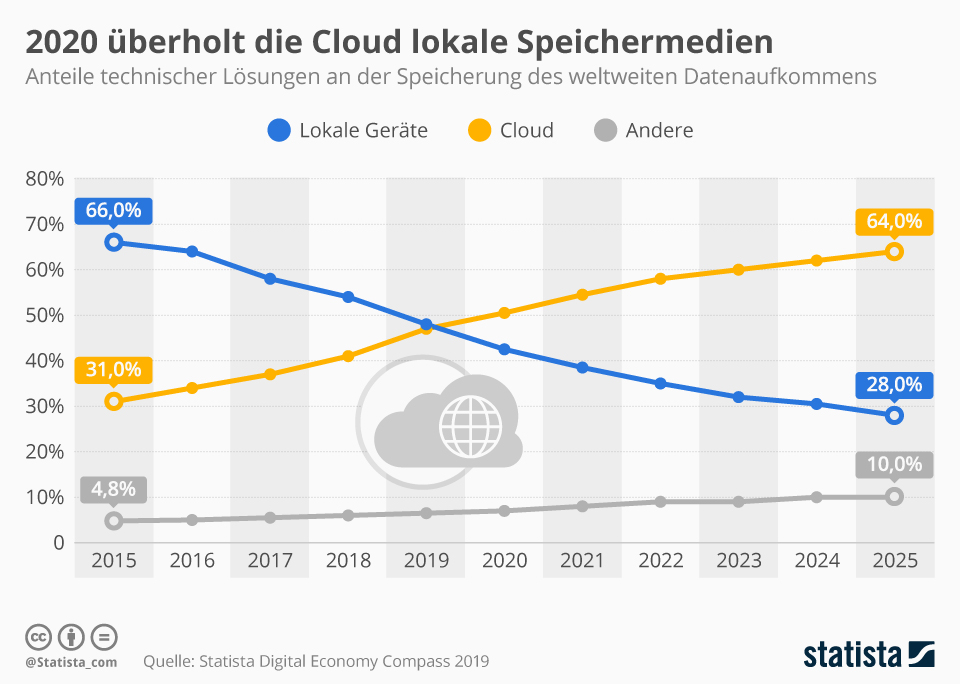
\includegraphics[scale=0.4]{sources/moreCloudStorageThanLocal}
      \caption[2020 überholt die Cloud lokale Speichermedien]{}\label{fig:moreCloudStorageThanLocal}
      2020 überholt die Cloud lokale Speichermedien
            %Quelle: Eigene Darstellung. 
            {\cite{STA1}}
\end{figure}

[ABSCHLUSS DES KAPITELS]
\newpage


\begin{comment}
Advantages of Cloud Technology
As the technology has matured over the last decade, companies are moving to the
cloud to lower costs, reduce complexity, and increase flexibility. The cloud
provides scalable and powerful compute solutions, low-cost, reliable storage, and addition, cloud technologies can be used to deploy solutions quickly and cost effectively around the world and on any device.
When you decouple from the data center, you’ll be able to:
x Decrease your TCO: Eliminate many of the costs related to building and
maintaining a data center or colocation deployment. Pay for only the
resources you consume.

x Reduce complexity: Reduce the need to manage infrastructure,
investigate licensing issues, or divert resources.
x Adjust capacity on the fly: Add or reduce resources, depending on
seasonal business needs, using infrastructure that is secure, reliable, and
broadly accessible.
x Reduce time to market: Design and develop new IT projects faster.
x Deploy quickly, even worldwide: Deploy applications across multiple
geographic areas.
x Increase efficiencies: Use automation to reduce or eliminate IT
management activities that waste time and resources.
x Innovate more: Spin up a new server and try out an idea. Each project
moves through the funnel more quickly because the cloud makes it faster
(and cheaper) to deploy, test, and launch new products and services.
x Spend your resources strategically: Switch to a DevOps model to free
your IT staff from operations and maintenance that can be handled by the
cloud services provider.
x Enhance security: Spend less time conducting security reviews on
infrastructure. Mature cloud providers have teams of people who focus on
security, offering best practices to ensure you’re compliant, no matter what
your industry.
\end{comment}

%\subsection{Was ist EC2? To Review}\label{subsec_UabsGrund4}
%Man kann HW und SW auswählen


% Amazon video Cloud Eco.: https://www.youtube.com/watch?v=kUNBx1MTwxw
% short explaniation https://www.youtube.com/watch?v=RI9RTbXEjLc
%3- Hard and Soft Savings https://youtu.be/Q5wSvUVPyYY?t=316
% Suche ein Buch, mit info darüber!

